\documentclass[10pt]{beamer}
\usetheme{Boadilla}
\usepackage[utf8]{inputenc}
\usepackage{amsmath}
\usepackage{amsfonts}
\usepackage{multicol}
\usepackage{listings}
\usepackage{sansmathaccent}
%\pdfmapfile{+sansmathaccent.map}
\usepackage{hyperref}
\usepackage{amssymb}
\DeclareGraphicsExtensions{,.pdf,.png,.jpg,.gif}
\usepackage{graphicx}
\setbeamercovered{transparent} 
\newcommand{\norm}[1]{\left\lVert#1\right\rVert}

\title[] %optional
{\huge {Procedimiento de vecinos más cercanos con matrices de distancias parcialmente observadas}}
 
\author[Aldo R. Franco Comas] % (optional, for multiple authors)
{\Large {Aldo R. Franco Comas}\\ 
\vspace{1cm}
{Director: Andrés M. Alonso}} 

\institute[UC3M] 

%\titlegraphic{\includegraphics[width=1.5cm]{imagenes/logo_uc3m.jpg}}
 
\date[Septiembre, 2018] % (optional)
{Máster Universitario en Ingeniería Matemática.}
 
\begin{document}

\begin{frame}
\titlepage
\end{frame}

\begin{frame}{Motivación}

\begin{block}{k-NN}
\begin{itemize}
    \item $\left\lbrace (x_i,y_i) \right\rbrace$ con $x_i$ de longitud $p$.
    \item Sea $x_{0}$ un nuevo caso, se calculan las distancias $d(x_0,x_i)$ para todo $i=1,...,n$.
    \item Se buscan los $k$ casos más cercanos.
\end{itemize}
\end{block}

\begin{block}{k-NN Ventajas}
	\begin{multicols}{2}
		\begin{itemize}
		\item No paramétrico.
		\item Algoritmo simple.
		\item Alta precisión.
		\item Múltiples clases.
		\item Clasificación y regresión.
		\item Variedad de distancias.
		\end{itemize}
	\end{multicols}
\end{block}

\begin{block}{KNN Desventajas}
	\begin{multicols}{2}
		\begin{itemize}
			\item Datos no balanceados.
			\item Computacionalmente costoso.
			\item Características homogéneas.
			\item Tratamiento con valores perdidos.
		\end{itemize}
	\end{multicols}
\end{block}

\end{frame}

\begin{frame}{Objetivos}

\begin{block}{¿Qué se propone?}
	\item Un procedimiento k-NN donde no sea necesario calcular todas las distancias  cada vez que tengamos que predecir un  punto. 
	
	Supondremos que solo podemos calcular $(1-\ell)\%$ de dichas distancias.
\end{block}

\begin{block}{¿Por qué?}
Es posible que no sea factible calcular todas esas distancias:
    \begin{itemize}
	    \item Tiempo de respuesta.
	    \item Coste computacional.
	    \item Pruebas destructivas.
	\end{itemize}
\end{block}

\begin{alertblock}{Repositorio}
\url{https://github.com/aldofranco91/TFM\_Ing\_Mat}
\end{alertblock}

\end{frame}

\begin{frame}{Definiciones básicas}

\begin{block}{}
\begin{itemize}
    \item Distancia euclidiana: $d_2(x,y) = \sqrt{\sum_{i=1}^{n}(x_i-y_i)^2}$ 
    \item Desigualdad triangular:  $m_{ik} \leq m_{ij} + m_{jk}$
     \item Desigualdad cuadrangular: $m_{ij} + m_{kl} \leq \max[m_{ik}+m_{jl} ; m_{il}+m_{jk}]$ 
    \item Desigualdad ultramétrica: $m_{ij} \leq \max[m_{ik};m_{jk}] $
    \item Error medio absoluto: $ \dfrac{\sum_{i=1}^{k}\left| \widehat{O}_{i} - O_{i}\right|}{k} $
    \item Diferencia relativa entre matrices: $\dfrac{\norm{O-P}_2}{\norm{O}_2}$
     \item Diferencia relativa entre vectores: $\dfrac{\norm{o-p}_2}{\norm{o}_2}$
    \item Índice de Jaccard: $\dfrac{\left| A \cap B \right| }{\left| A \cup B \right|}$
\end{itemize}
\end{block}
\end{frame}

\begin{frame}{Revisión de la literatura}

\begin{block}{Completamiento de matrices de distancias}
\begin{itemize}
    \item Problema de la métrica más cercana.
    \item Problema de la inferencia filogenética.
\end{itemize}
\end{block}

\begin{block}{Relación entre el k-NN propuesto y el completamiento de matrices de distancias}
\begin{itemize}
    \item Asumimos que conocemos la matriz de distancia entre los $n$ puntos de la muestra de entrenamiento.
    \item Creamos una nueva matriz de distancias $(n+1) \times (n+1)$, siendo la última fila/columna la correspondiente a $x_0$.
    \item Calculamos $(1-\ell)\%$ de las distancias de esa fila, las restantes las imputamos.
\end{itemize}
\end{block}

\end{frame}

\begin{frame}{Problema de la métrica más cercana}

\begin{block}{}
Supongamos que tenemos una matriz $\pmb{D}$ cuyos elementos deben cumplir las desigualdades triangulares pero en algunos casos no se verifican. \vspace{0.25cm}

El \alert{problema de la métrica más cercana} consiste en encontrar una matriz $\pmb{M}$ cuyos elementos cumplan las desigualdades triangulares y que esté próxima a $\pmb{D}$. \vspace{0.25cm}

El \alert{algoritmo triangle fixing} resuelve este problema para las metricas $L_1$, $L_2$ y $L_\infty$.
\end{block}

\begin{block}{Inicialización del algoritmo}
\begin{itemize}
	\item $d(x_0,x_j) = 0$
	\item $d(x_0,x_j) = n^{-1} \sum\limits_{i=1}^{n}d(x_i,x_j)  \quad , i \neq j$
	\item $d(x_0,x_j) = \text{mediana}(d(x_i,x_j)) \quad , \forall i \neq j$
\end{itemize}
\end{block}
\end{frame}

\begin{frame}{Problema de la métrica más cercana}

\only<1>{

\begin{block}{Ejercicio de simulación}
\begin{enumerate}
	\item Se generan $n = 800$ puntos de una distribución normal multivariante con $\mu = \vec{0}_p$ y $\sigma = I_p$, siendo $p=20$. 
	\item Se calcula la matriz de distancias, $\pmb{\mathcal{D}}$, usando la distancia euclidiana.
	\item Se genera un nuevo punto $x_0$ y se calculan las $n$ distancias.
	\item Se asumen conocidas las distancias de $x_0$ a $n(1-\ell) = 80$ puntos al azar y las restantes distancias se imputan usando las distintas inicializaciones, con lo cual tenemos una matriz $\pmb{D}$.
	\item Se aplica el triangle fixing a $\pmb{D}$ y nos devuelve una matriz $\pmb{M}$.
	\item Se calcula la diferencia relativa entre la matriz $\pmb{M}$ y la matriz $\pmb{\mathcal{D}}$ y la diferencia relativa entre el vector de distancias correspondiente a $x_0$ en la matriz $\pmb{\mathcal{D}}$ y en $\pmb{M}$. Se registra el tiempo de cómputo.
	\item Todo lo anterior se hace $N = 2000$ veces.
\end{enumerate}
\end{block}

}

\only<2>{
\begin{figure}[H]
	\centering
	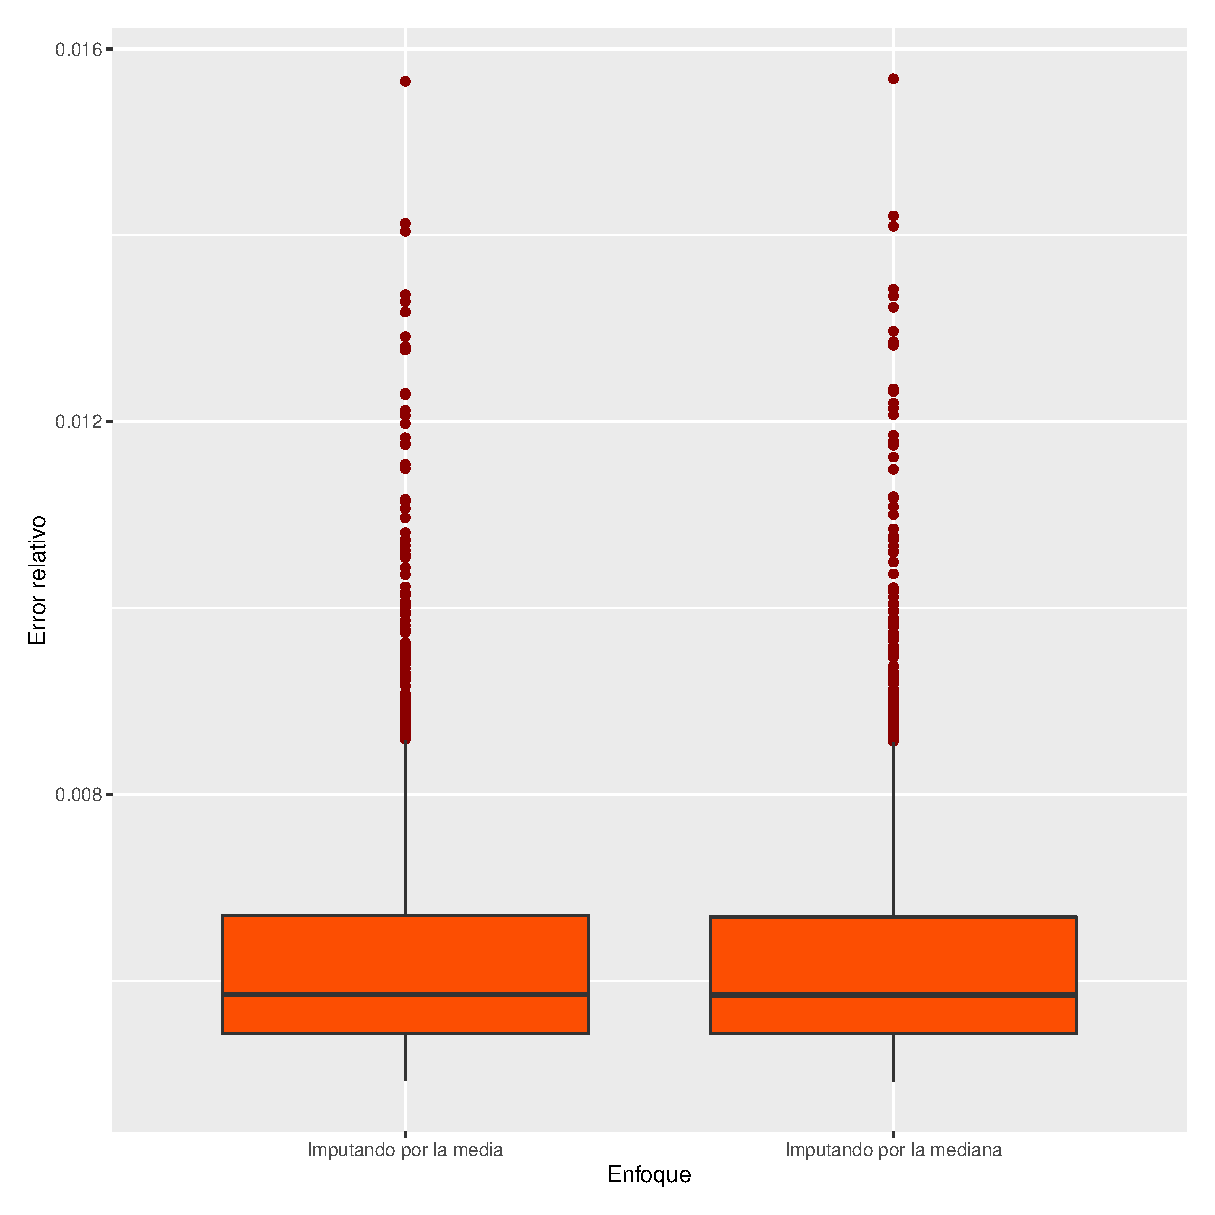
\includegraphics[scale=0.345]{imagenes/tf_imputation_mean_and_median_dif_relativa.eps}
\end{figure}
\centering Diagramas de caja de las diferencias relativas entre $\pmb{\mathcal{D}}$ y $\pmb{M}$
}

\only<3>{
\begin{figure}[H]
	\centering
	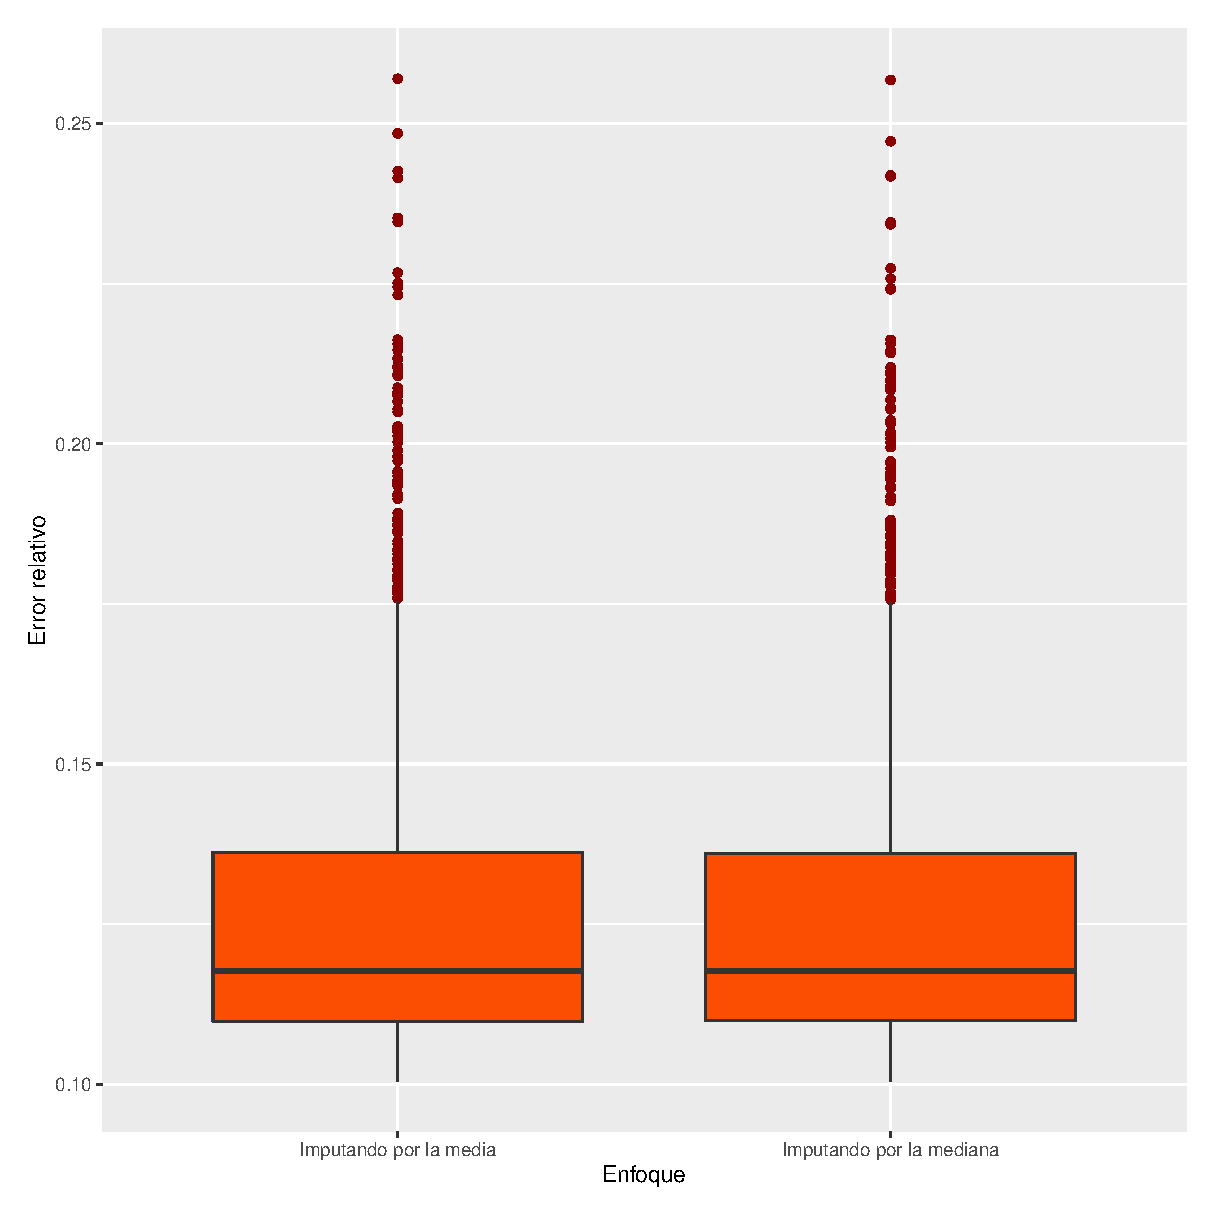
\includegraphics[scale=0.345]{imagenes/tf_imputation_mean_and_median_errores.eps}
\end{figure}
\centering Diagramas de caja de las diferencias relativas entre vectores de distancia.
}

\only<4>{
\begin{figure}[H]
	\centering
	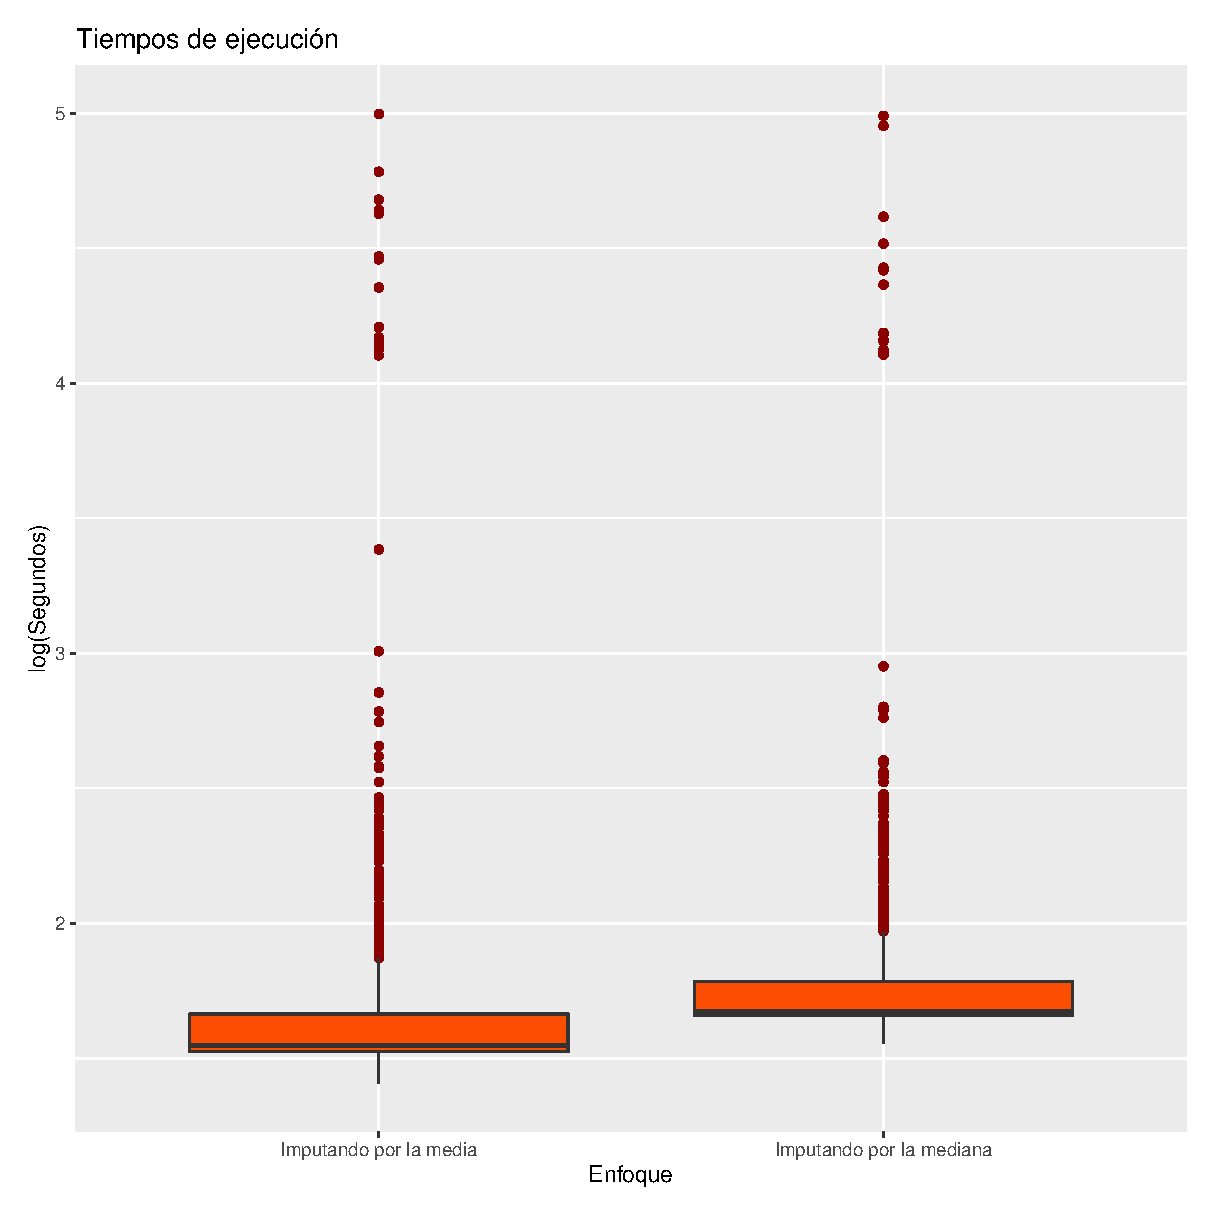
\includegraphics[scale=0.3]{imagenes/tf_imputation_mean_and_median_tiempo.eps}
\end{figure}
\centering Diagramas de caja de los tiempos de computo.
}

\end{frame}

\begin{frame}{Problema de la métrica más cercana: Método propuesto}

\only<1>{
\begin{block}{Restricciones}
\begin{itemize}
	\item Las distancias $d(x_i,x_j)$ son conocidas $\forall i,j=\left\lbrace 1,...,n\right\rbrace$.
	\item Podemos calcular las distancias de $d(x_0,x_i)$ cuando $i \in I$ y $\left| I \right| << n$.
	\item No podemos calcular las $d(x_0,x_i)$ cuando $i \in I^c$.
	\item $\left| I \right| \approx (1-\ell)n$ y $\left| I^c \right| \approx \ell n$.  
\end{itemize}
\end{block}
}

\only<2>{
\begin{block}{Acotación}
$$ d(x_0,x_{i^*}) \leq d(x_0,x_i) + d(x_i,x_{i^*}) \quad \forall i^* \in I^c $$
\alert{$$ d(x_0,x_{i^*}) \leq \min_{i \in I} \left\lbrace d(x_0,x_i) + d(x_i,x_{i^*}) \right\rbrace  $$}
$$ d(x_i,x_{i^*}) \leq d(x_0,x_{i^*}) + d(x_0,x_{i}) \quad \forall i^* \in I^c $$
$$ d(x_0,x_{i}) \leq d(x_0,x_{i^*}) + d(x_i,x_{i^*}) \quad \forall i^* \in I^c $$
\alert{$$ \max_{i \in I} \left| d(x_0,x_{i}) - d(x_i,x_{i^*}) \right| \leq d(x_0,x_{i^*}) $$}
$$ \max_{i \in I} \left| d(x_0,x_{i}) - d(x_i,x_{i^*}) \right| \leq d(x_0,x_{i^*}) \leq  \min_{i \in I} \left\lbrace d(x_0,x_i) + d(x_i,x_{i^*}) \right\rbrace $$
\end{block}
\begin{block}{}\vspace{-0.35cm}
$$d(x_0,x_{i^*}) = \dfrac{1}{2} \left( \min_{i \in I} \left\lbrace d(x_0,x_i) + d(x_i,x_{i^*}) \right\rbrace + \max_{i \in I} \left| d(x_0,x_{i}) - d(x_i,x_{i^*}) \right| \right)$$
\end{block}
}

\end{frame}

\begin{frame}{Problema de la métrica más cercana: Clúster}

\begin{block}{Análisis de grupos}
\begin{itemize}
    \item Técnica de aprendizaje no supervisada.
    \item Objetos dentro del mismo clúster son similares.
\end{itemize}
\end{block}

\begin{block}{Algoritmos para clúster:}
\begin{itemize}
    \item Agrupamiento jerárquico:
    \begin{itemize}
        \item Aglomerativo
        \item Divisivo.
    \end{itemize}
    \item Agrupamiento no jerárquico:
    \begin{itemize}
        \item K-medias.
        \item K-medoides:
        \begin{itemize}
            \item PAM
            \item CLARA, CLARANS
            \item \alert{fastkmed}
        \end{itemize}
    \end{itemize}
\end{itemize}
\end{block}

    
\end{frame}

\begin{frame}{Selección de K}

\only<1>{
\begin{block}{}
\begin{enumerate}
	 \item Se generan $n = 3000$ puntos de una distribución normal multivariante con $\mu = \vec{0}_p$ y $\sigma = I_p$, siendo $p=50$.
	 \item Se calcula la matriz de distancias, $\pmb{\mathcal{D}}$, usando la distancia euclidiana.
	 \item Se aplica $fastkmed$ a $\pmb{\mathcal{D}}$ para diferentes valores de $K = (2,4,8,16,32,64,150,300) $ y se obtienen $K$ mediodes $\left\lbrace C_1,...,C_K\right\rbrace $.
	 \item Se genera un nuevo punto $x_0$.
	 \item Se calculan y ordenan las distancias $d(x_0,C_i)$ con $i=1,...,K$.
	 \item  En este punto ya hemos calculado $K$ distancias y se calculan las restantes hasta $n(1-\ell) = 300$ distancias a puntos en los clústeres más cercanos.
	 \item Para los diferentes valores de $K$ expuestos se calcula el índice de Jaccard y el MAE entre el conjunto real de puntos más cercano y el conjunto de puntos más cercano que se obtiene imputando, para $k=15$ vecinos.
	 \item Los pasos $4-7$ se repiten $N=200$ veces.
\end{enumerate}
\end{block}
}

\only<2>{
\begin{figure}[H]
	\centering
	\includegraphics[scale=0.50]{imagenes/{cluster_fastmed_knn_fijo_cluster_varia}.eps}
\end{figure}
\centering Búsqueda de un valor ``óptimo'' de clústeres.
$$ K = (n-\ell n)/2 $$
}
\end{frame}

\begin{frame}{Selección al azar vs. Clúster}

\only<1>{
\begin{block}{}
\begin{enumerate}
	 \item Se generan $n=5000$ puntos de una distribución normal multivariante con $\mu = \vec{0}_p$ y $\sigma = I_p$, siendo $p=50$.
	 \item Se calcula la matriz de distancias, $\pmb{\mathcal{D}}$, usando la distancia euclidiana.
	 \item Se genera un nuevo punto $x_0$.
	\item Se calculan las distancias de $x_0$ a los $n$ puntos. 
	\item Se calculan las distancias de $x_0$ a $n(1-\ell)$ puntos al azar y también a la misma cantidad usando $K = (n-ln)/2$ clústeres. 
	 \item Se ordenan dichas distancias y se extrae cuáles son los $k$ puntos más cercanos, el máximo valor que toma $k$ es $\sqrt{n}/2$.
	\item Para diferentes valores de $k$ se calcula el índice de Jaccard y el MAE.
	\item Los pasos $4-7$ se repiten $N=1000$ veces.
\end{enumerate}
\end{block}
}

\only<2>{
\begin{figure}[H]
	\centering
	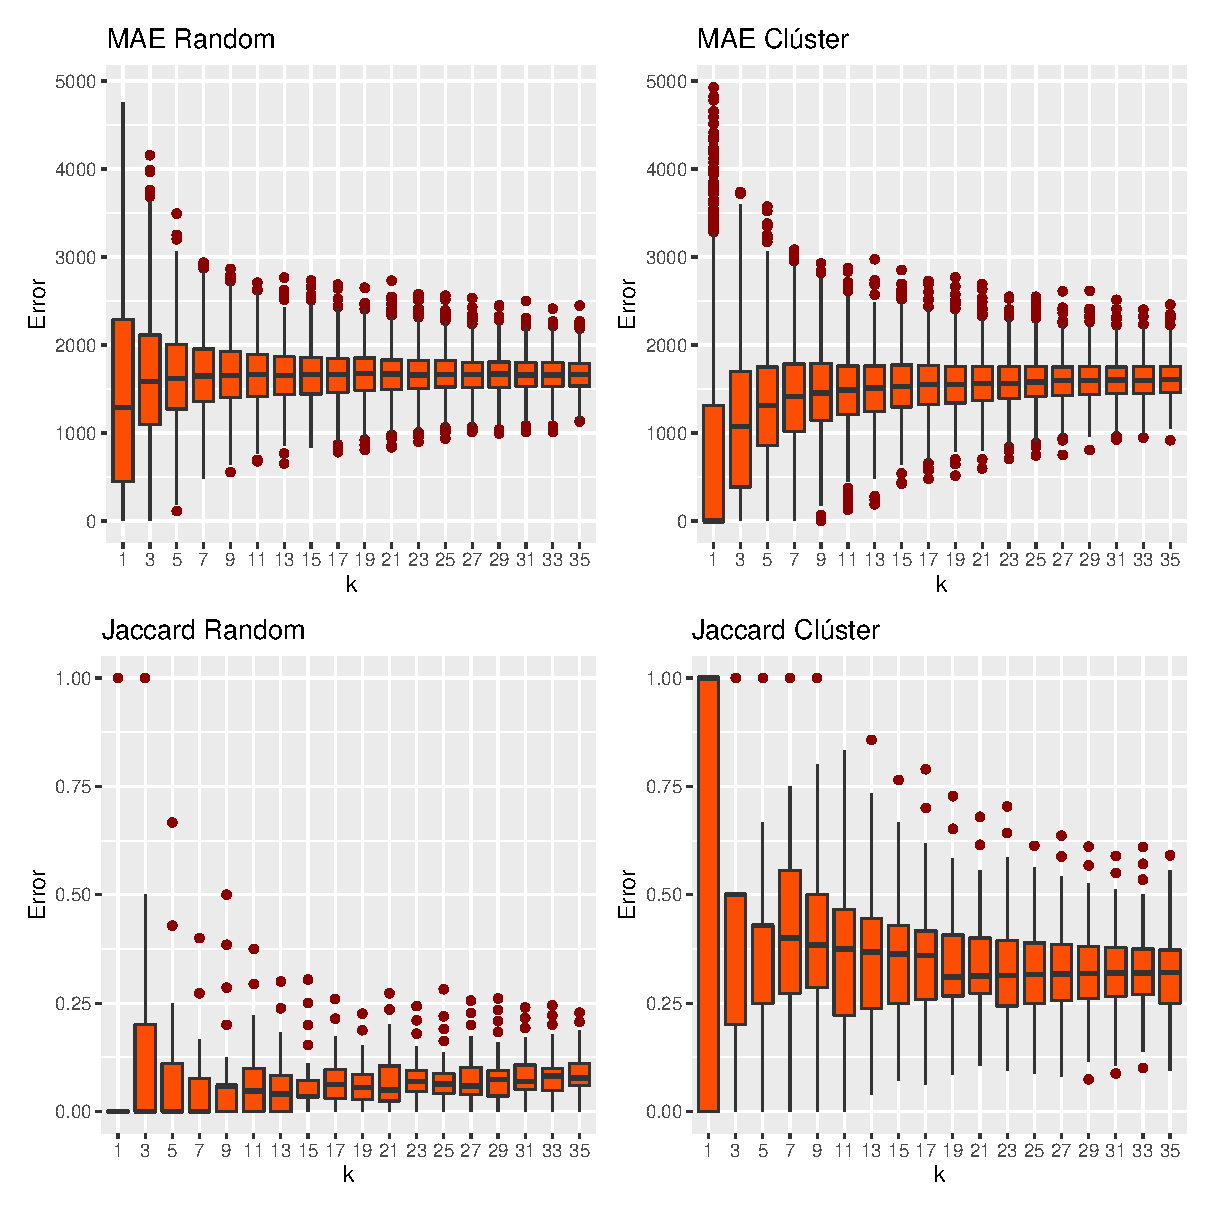
\includegraphics[scale=0.4]{imagenes/our_random_vs_our_cluster_fastmed.eps}
\end{figure}
}

\end{frame}


\begin{frame}{Aditivo vs. Ultramétrica}
    \begin{figure}[H]
	\centering
	\includegraphics[scale=0.35]{imagenes/{Ultrametric_Additive}.eps}
\end{figure}
\centering $n=1000$, $l=90\%$, $p=20$ y $N = 300$.
\end{frame}

\begin{frame}{Ultramétrica vs. Agrupamiento}

\begin{figure}[H]
	\centering
	\includegraphics[scale=0.35]{imagenes/{our_and_ultrametric}.eps}
\end{figure}
\centering $n=1000$, $l=90\%$, $p=20$ y $N = 300$.
\end{frame}

\begin{frame}{MNIST}

\only<1>{
Imágenes en blanco y negro (42000) normalizadas cuyas dimensiones son de 28x28 píxeles en niveles de escala de grises de dígitos escritos a mano. \vspace{0.25cm}

El problema de clasificación, consiste en, dada una nueva imagen debemos predecir que número tiene escrito.
    \begin{figure}[H]
	\centering
	\includegraphics[scale=0.4]{imagenes/mnist.png}
	\end{figure}
}

\only<2>{
El 75$\%$ de las imágenes se utiliza para entrenar y el 25\% restante de prueba. Esta división se hizo usando un reparto estratificado entre las muestras de entrenamiento y de prueba.

\begin{figure}[H]
	\centering
	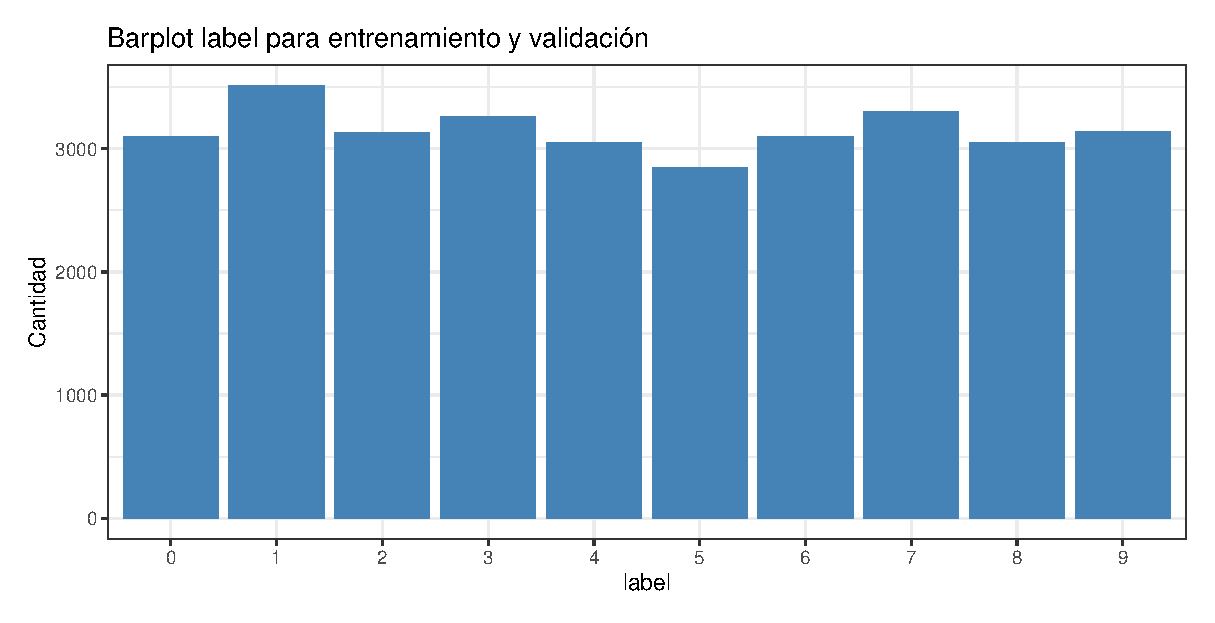
\includegraphics[scale=0.3]{imagenes/mnisttrain.eps}
\end{figure}

\begin{figure}[H]
	\centering
	\includegraphics[scale=0.3]{imagenes/mnisttest.eps}
\end{figure}
}

\only<3>{
\begin{figure}[H]
	\centering
	\includegraphics[scale=0.34]{imagenes/knn.png}
\end{figure}
\centering Validación cruzada con 5 submuestras, se obtiene una precisión del $96.14\%$.
}

\only<4>{
Matriz de confusión usando k-NN($k=3$).
\begin{table}[H]\small
	\centering
	\begin{tabular}{|c|c|c|c|c|c|c|c|c|c|c|}
		\hline
		& \multicolumn{10}{c|}{Valor Real}                                 \\ \hline
		Predicción & 0    & 1    & 2    & 3    & 4   & 5   & 6    & 7    & 8   & 9    \\ \hline
		0          & 1024 & 0    & 4    & 2    & 1   & 4   & 6    & 2    & 1   & 6    \\ \hline
		1          & 0    & 1161 & 8    & 1    & 7   & 1   & 0    & 6    & 10  & 2    \\ \hline
		2          & 2    & 4    & 1002 & 4    & 0   & 2   & 2    & 3    & 4   & 2    \\ \hline
		3          & 1    & 0    & 5    & 1043 & 0   & 8   & 1    & 0    & 18  & 10   \\ \hline
		4          & 0    & 1    & 0    & 0    & 985 & 0   & 0    & 1    & 3   & 8    \\ \hline
		5          & 0    & 1    & 1    & 20   & 0   & 920 & 6    & 0    & 16  & 6    \\ \hline
		6          & 5    & 0    & 0    & 1    & 8   & 11  & 1019 & 0    & 5   & 0    \\ \hline
		7          & 0    & 3    & 21   & 5    & 3   & 0   & 0    & 1083 & 5   & 10   \\ \hline
		8          & 0    & 1    & 1    & 6    & 1   & 0   & 0    & 0    & 941 & 1    \\ \hline
		9          & 1    & 0    & 2    & 5    & 13  & 2   & 0    & 5    & 12  & 1002 \\ \hline
	\end{tabular}
\end{table}
\centering Precisión: $96.98\%$
}

\only<5>{
Matriz de confusión usando imputación mediante clústeres con $l = 0.75$.
\begin{table}[H]\small
	\centering
	\begin{tabular}{|c|c|c|c|c|c|c|c|c|c|c|}
		\hline
		& \multicolumn{10}{c|}{Valor Real}                                \\ \hline
		Predicción & 0    & 1    & 2   & 3    & 4   & 5   & 6    & 7    & 8   & 9    \\ \hline
		0          & 1022 & 0    & 9   & 3    & 2   & 4   & 11   & 0    & 4   & 4    \\ \hline
		1          & 1    & 1166 & 10  & 4    & 10  & 2   & 1    & 10   & 11  & 1    \\ \hline
		2          & 1    & 1    & 990 & 7    & 0   & 0   & 1    & 6    & 7   & 0    \\ \hline
		3          & 0    & 1    & 2   & 1030 & 0   & 7   & 0    & 0    & 14  & 3    \\ \hline
		4          & 1    & 2    & 2   & 0    & 971 & 0   & 2    & 6    & 4   & 6    \\ \hline
		5          & 0    & 0    & 0   & 14   & 0   & 920 & 2    & 0    & 19  & 2    \\ \hline
		6          & 6    & 0    & 4   & 3    & 7   & 8   & 1016 & 0    & 11  & 1    \\ \hline
		7          & 2    & 0    & 21  & 13   & 4   & 2   & 0    & 1067 & 5   & 12   \\ \hline
		8          & 0    & 0    & 3   & 7    & 0   & 1   & 1    & 0    & 923 & 2    \\ \hline
		9          & 0    & 1    & 3   & 6    & 24  & 4   & 0    & 11   & 17  & 1016 \\ \hline
	\end{tabular}
\end{table}
\centering Precisión: $96.42\%$
}
\end{frame}

\begin{frame}{DIAMONDS}
\only<1>{
\begin{block}{}
\begin{itemize}
    \item Precios y otros diez atributos de casi $54000$ diamantes.
    \item  Minimizar el error absoluto medio de la predicción del precio en función de los atributos del diamante. 
\end{itemize}
\end{block}

\begin{itemize}
	\item \underline{price:} Precio en USD.
	\item \underline{carat:} Peso en quilates del diamante.
	\item \underline{cut:} Calidad del corte.
	\item \underline{color:} Color del diamante.
	\item \underline{clarity:} Claridad del diamante.
	\item \underline{x:} Longitud en mm.
	\item \underline{y:} Ancho en mm.
	\item \underline{z:} Profundidad en mm.
	\item \underline{profundidad:} Porcentaje de profundidad total.
	\item \underline{depth:} Ancho de la parte superior en relación con el punto más ancho.
	\item \underline{table:} Ancho de la parte superior del diamante.
\end{itemize}
}

\only<2>{
\begin{figure}[H]
	\centering
	\includegraphics[scale=0.3]{imagenes/knn2.png}
\end{figure}

\begin{block}{}
\begin{itemize}
    \item 75$\%$ para entrenamiento y 25\% para prueba.
    \item $k = 3$ es el mejor parámetro, $MAE = 448.2$. 
    \item $MAE = 432.881$ usando k-NN en los datos de prueba.
    \item $MAE = 531.35$ usando el método propuesto con $l=0.75$.
    \item $MAE = 639.83$ usando k-NN con muestra de entrenamiento del 25\%.
\end{itemize}
\end{block}
}

\only<3>{
Comparación de una muestra entre k-NN, imputación mediante clústeres y valores reales de DIAMONDS
\begin{figure}[H]
	\centering
	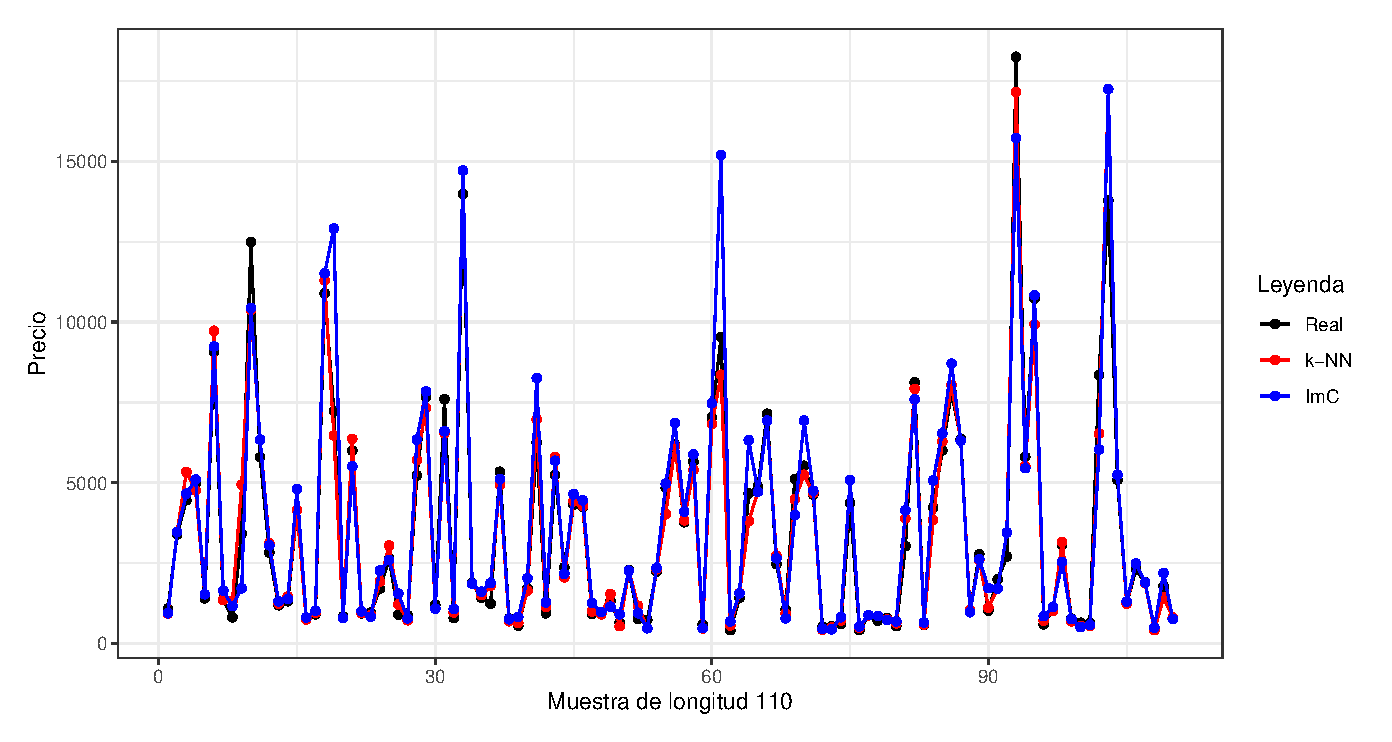
\includegraphics[scale=0.5]{imagenes/finaldiamonds.eps}
\end{figure}
}
\end{frame}

\begin{frame}{Conclusiones y extensiones}

\begin{block}{Conclusiones}
\begin{itemize}
     \item Modificaciones al procedimiento k-NN y estudiado el algoritmo triangle fixing con varias opciones de inicialización.
     \item Observaciones al azar en el conjunto de entrenamiento es inferior a una selección basada en clústeres.
     \item El procedimiento de imputación basado en clústeres es superior a los algoritmos aditivos y ultramétricos.
     \item Conjuntos de datos reales que muestran que en problemas de clasificación los resultados son similares al k-NN cosa que no ocurre con el problema de regresión.
\end{itemize}
\end{block}


\begin{block}{Extensiones}
\begin{itemize}
 \item Implementar estos algoritmos en un lenguaje como \textbf{\textsf{C}} o \textbf{\textsf{C++}}.
 \item Buscar un número ``óptimo'' de clústeres, $K$.
 \item Selección conjunta del parámetro $k$ del k-NN y del parámetro $K$ del procedimiento de imputación mediante clústeres.
\end{itemize}
\end{block}


\end{frame}

\begin{frame}
\begin{center}
{\Huge Muchas Gracias}
\end{center}
\end{frame}

\end{document}

